% ****************************************************************************************
% ************************              ADOO                  ****************************
% ****************************************************************************************


% =======================================================
% =======         HEADER FOR DOCUMENT        ============
% =======================================================
    
    % *********   HEADERS AND FOOTERS ********
    \def\ProjectAuthorLink{https://github.com/SoyOscarRH}           %Just to keep it in line
    \def\ProjectNameLink{\ProjectAuthorLink/Proyect}                %Link to Proyect

    % *********   DOCUMENT ITSELF   **************
    \documentclass[12pt, fleqn]{report}                             %Type of document and size of font and left eq
    \usepackage[spanish]{babel}                                     %Please use spanish
    \usepackage[utf8]{inputenc}                                     %Please use spanish - UFT
    \usepackage[margin = 1.2in]{geometry}                           %Margins and Geometry pacakge
    \usepackage{ifthen}                                             %Allow simple programming
    \usepackage{hyperref}                                           %Create MetaData for a PDF and LINKS!
    \usepackage{pdfpages}                                           %Create MetaData for a PDF and LINKS!
    \hypersetup{pageanchor = false}                                 %Solve 'double page 1' warnings in build
    \setlength{\parindent}{0pt}                                     %Eliminate ugly indentation
    \author{Oscar Rosas, Alan Ontiveros y Laura Morales}            %Who I am

    % *********   LANGUAJE    *****************
    \usepackage[T1]{fontenc}                                        %Please use spanish
    \usepackage{textcmds}                                           %Allow us to use quoutes
    \usepackage{changepage}                                         %Allow us to use identate paragraphs
    \usepackage{anyfontsize}                                        %All the sizes

    % *********   MATH AND HIS STYLE  *********
    \usepackage{ntheorem, amsmath, amssymb, amsfonts}               %All fucking math, I want all!
    \usepackage{mathrsfs, mathtools, empheq}                        %All fucking math, I want all!
    \usepackage{cancel}                                             %Negate symbol
    \usepackage{centernot}                                          %Allow me to negate a symbol
    \decimalpoint                                                   %Use decimal point

    % *********   GRAPHICS AND IMAGES *********
    \usepackage{graphicx}                                           %Allow to create graphics
    \usepackage{float}                                              %For images
    \usepackage{wrapfig}                                            %Allow to create images
    \graphicspath{ {Graphics/} }                                    %Where are the images :D

    % *********   LISTS AND TABLES ***********
    \usepackage{listings, listingsutf8}                             %We will be using code here
    \usepackage[inline]{enumitem}                                   %We will need to enumarate
    \usepackage{tasks}                                              %Horizontal lists
    \usepackage{longtable}                                          %Lets make tables awesome
    \usepackage{booktabs}                                           %Lets make tables awesome
    \usepackage{tabularx}                                           %Lets make tables awesome
    \usepackage{multirow}                                           %Lets make tables awesome
    \usepackage{multicol}                                           %Create multicolumns

    % *********   HEADERS AND FOOTERS ********
    \usepackage{fancyhdr}                                           %Lets make awesome headers/footers
    \pagestyle{fancy}                                               %Lets make awesome headers/footers
    \setlength{\headheight}{16pt}                                   %Top line
    \setlength{\parskip}{0.5em}                                     %Top line
    \renewcommand{\footrulewidth}{0.5pt}                            %Bottom line

    \lhead {                                                        %Left Header
        \hyperlink{chapter.\arabic{chapter}}                        %Make a link to the current chapter
        {\normalsize{\textsc{\nouppercase{\leftmark}}}}         \textbf{}    %And fot it put the name
    }

    \rhead {                                                        %Right Header
        \hyperlink{section.\arabic{chapter}.\arabic{section}}       %Make a link to the current chapter
            {\footnotesize{\textsc{\nouppercase{\rightmark}}}}      %And fot it put the name
    }

    \rfoot{\textsc{\small{\hyperref[sec:Index]{Ve al Índice}}}}     %This will always be a footer  

    \fancyfoot[L]{                                                  %Algoritm for a changing footer
        \ifthenelse{\isodd{\value{page}}}                           %IF ODD PAGE:
            {\href{https://compilandoconocimiento.com/nosotros/}    %DO THIS:
                {\tiny                                              %Send the page
                    {\textsc{                                       %Send the page
                    Oscar Rosas, Alan Ontiveros y Laura Morale}}}}  %Send the page
            {\href{https://compilandoconocimiento.com}              %ELSE DO THIS: 
                {\footnotesize                                      %Send the author
                    {\textsc{T de Tiendita}}}}                      %Send the author
    }
    
    \usepackage{gantt}
    \definecolor{barblue}{RGB}{153,204,254}
\definecolor{groupblue}{RGB}{51,102,254}
\definecolor{linkred}{RGB}{165,0,33} 
    
% =======================================================
% ===================   COMMANDS    =====================
% =======================================================

    % =========================================
    % =======   NEW ENVIRONMENTS   ============
    % =========================================
    \newenvironment{Indentation}[1][0.75em]                         %Use: \begin{Inde...}[Num]...\end{Inde...}
        {\begin{adjustwidth}{#1}{}}                                 %If you dont put nothing i will use 0.75 em
        {\end{adjustwidth}}                                         %This indentate a paragraph
    \newenvironment{SmallIndentation}[1][0.75em]                    %Use: The same that we upper one, just 
        {\begin{adjustwidth}{#1}{}\begin{footnotesize}}             %footnotesize size of letter by default
        {\end{footnotesize}\end{adjustwidth}}                       %that's it

    \newenvironment{MultiLineEquation}[1]                           %Use: To create MultiLine equations
        {\begin{equation}\begin{alignedat}{#1}}                     %Use: \begin{Multi..}{Num. de Columnas}
        {\end{alignedat}\end{equation}}                             %And.. that's it!
    \newenvironment{MultiLineEquation*}[1]                          %Use: To create MultiLine equations
        {\begin{equation*}\begin{alignedat}{#1}}                    %Use: \begin{Multi..}{Num. de Columnas}
        {\end{alignedat}\end{equation*}}                            %And.. that's it!
    

    % =========================================
    % == GENERAL TEXT & SYMBOLS ENVIRONMENTS ==
    % =========================================
    
    % =====  TEXT  ======================
    \newcommand \Quote {\qq}                                        %Use: \Quote to use quotes
    \newcommand \Over {\overline}                                   %Use: \Bar to use just for short
    \newcommand \ForceNewLine {$\Space$\\}                          %Use it in theorems for example

    % =====  SPACES  ====================
    \DeclareMathOperator \Space {\quad}                             %Use: \Space for a cool mega space
    \DeclareMathOperator \MegaSpace {\quad \quad}                   %Use: \MegaSpace for a cool mega mega space
    \DeclareMathOperator \MiniSpace {\;}                            %Use: \Space for a cool mini space
    
    % =====  MATH TEXT  =================
    \newcommand \Such {\MiniSpace | \MiniSpace}                     %Use: \Such like in sets
    \newcommand \Also {\MiniSpace \text{y} \MiniSpace}              %Use: \Also so it's look cool
    \newcommand \Remember[1]{\Space\text{\scriptsize{#1}}}          %Use: \Remember so it's look cool
    
    % =====  THEOREMS  ==================
    \newtheorem{Theorem}{Teorema}[section]                          %Use: \begin{Theorem}[Name]\label{Nombre}...
    \newtheorem{Corollary}{Colorario}[Theorem]                      %Use: \begin{Corollary}[Name]\label{Nombre}...
    \newtheorem{Lemma}[Theorem]{Lemma}                              %Use: \begin{Lemma}[Name]\label{Nombre}...
    \newtheorem{Definition}{Definición}[section]                    %Use: \begin{Definition}[Name]\label{Nombre}...
    \theoremstyle{break}                                            %THEOREMS START 1 SPACE AFTER

    % =====  LOGIC  =====================
    \newcommand \lIff {\leftrightarrow}                             %Use: \lIff for logic iff
    \newcommand \lEqual {\MiniSpace \Leftrightarrow \MiniSpace}     %Use: \lEqual for a logic double arrow
    \newcommand \lInfire {\MiniSpace \Rightarrow \MiniSpace}        %Use: \lInfire for a logic infire
    \newcommand \lLongTo {\longrightarrow}                          %Use: \lLongTo for a long arrow

    % =====  FAMOUS SETS  ===============
    \DeclareMathOperator \Naturals     {\mathbb{N}}                 %Use: \Naturals por Notation
    \DeclareMathOperator \Primes       {\mathbb{P}}                 %Use: \Primes por Notation
    \DeclareMathOperator \Integers     {\mathbb{Z}}                 %Use: \Integers por Notation
    \DeclareMathOperator \Racionals    {\mathbb{Q}}                 %Use: \Racionals por Notation
    \DeclareMathOperator \Reals        {\mathbb{R}}                 %Use: \Reals por Notation
    \DeclareMathOperator \Complexs     {\mathbb{C}}                 %Use: \Complex por Notation
    \DeclareMathOperator \GenericField {\mathbb{F}}                 %Use: \GenericField por Notation
    \DeclareMathOperator \VectorSet    {\mathbb{V}}                 %Use: \VectorSet por Notation
    \DeclareMathOperator \SubVectorSet {\mathbb{W}}                 %Use: \SubVectorSet por Notation
    \DeclareMathOperator \Polynomials  {\mathbb{P}}                 %Use: \Polynomials por Notation

    % =====  CONTAINERS   ===============
    \newcommand{\Set}[1]{\left\{ \; #1 \; \right\}}                 %Use: \Set {Info} for INTELLIGENT space 
    \newcommand{\bigSet}[1]{\big\{ \; #1 \; \big\}}                 %Use: \bigSet  {Info} for space 
    \newcommand{\BigSet}[1]{\Big\{ \; #1 \; \Big\}}                 %Use: \BigSet  {Info} for space 
    \newcommand{\biggSet}[1]{\bigg\{ \; #1 \; \bigg\}}              %Use: \biggSet {Info} for space 
    \newcommand{\BiggSet}[1]{\Bigg\{ \; #1 \; \Bigg\}}              %Use: \BiggSet {Info} for space 
    
    \newcommand{\Brackets}[1]{\left[ #1 \right]}                    %Use: \Brackets {Info} for INTELLIGENT space
    \newcommand{\bigBrackets}[1]{\big[ \; #1 \; \big]}              %Use: \bigBrackets  {Info} for space 
    \newcommand{\BigBrackets}[1]{\Big[ \; #1 \; \Big]}              %Use: \BigBrackets  {Info} for space 
    \newcommand{\biggBrackets}[1]{\bigg[ \; #1 \; \bigg]}           %Use: \biggBrackets {Info} for space 
    \newcommand{\BiggBrackets}[1]{\Bigg[ \; #1 \; \Bigg]}           %Use: \BiggBrackets {Info} for space 
    
    \newcommand{\Wrap}[1]{\left( #1 \right)}                        %Use: \Wrap {Info} for INTELLIGENT space
    \newcommand{\bigWrap}[1]{\big( \; #1 \; \big)}                  %Use: \bigBrackets  {Info} for space 
    \newcommand{\BigWrap}[1]{\Big( \; #1 \; \Big)}                  %Use: \BigBrackets  {Info} for space 
    \newcommand{\biggWrap}[1]{\bigg( \; #1 \; \bigg)}               %Use: \biggBrackets {Info} for space 
    \newcommand{\BiggWrap}[1]{\Bigg( \; #1 \; \Bigg)}               %Use: \BiggBrackets {Info} for space 

    % =====  BETTERS MATH COMMANDS   =====
    \newcommand{\pfrac}[2]{\Wrap{\dfrac{#1}{#2}}}                   %Use: Put fractions in parentesis

    % =========================================
    % ====   LINEAL ALGEBRA & VECTORS    ======
    % =========================================

    % ===== UNIT VECTORS  ================
    \newcommand{\hati} {\hat{\imath}}                               %Use: \hati for unit vector    
    \newcommand{\hatj} {\hat{\jmath}}                               %Use: \hatj for unit vector    
    \newcommand{\hatk} {\hat{k}}                                    %Use: \hatk for unit vector

    % ===== MAGNITUDE  ===================
    \newcommand{\abs}[1]{\left\lvert #1 \right\lvert}               %Use: \abs{expression} for |x|
    \newcommand{\Abs}[1]{\left\lVert #1 \right\lVert}               %Use: \Abs{expression} for ||x||
    \newcommand{\Mag}[1]{\left| #1 \right|}                         %Use: \Mag {Info} 
    
    \DeclareMathOperator \LinealTransformation {\mathcal{T}}        %Use: \LinealTransformation for a cool T
    \newcommand{\bVec}[1]{\mathbf{#1}}                              %Use for bold type of vector
    \newcommand{\lVec}[1]{\overrightarrow{#1}}                      %Use for a long arrow over a vector
    \newcommand{\uVec}[1]{\mathbf{\hat{#1}}}                        %Use: Unitary Vector Example: $\uVec{i}

    % ===== ALL FOR DOT PRODUCT  =========
    \makeatletter                                                   %WTF! IS THIS
    \newcommand*\dotP{\mathpalette\dotP@{.5}}                       %Use: \dotP for dot product
    \newcommand*\dotP@[2] {\mathbin {                               %WTF! IS THIS            
        \vcenter{\hbox{\scalebox{#2}{$\m@th#1\bullet$}}}}           %WTF! IS THIS
    }                                                               %WTF! IS THIS
    \makeatother                                                    %WTF! IS THIS

    % === WRAPPERS FOR COLUMN VECTOR ===
    \newcommand{\pVector}[1]                                        %Use: \pVector {Matrix Notation} use parentesis
        { \ensuremath{\begin{pmatrix}#1\end{pmatrix}} }             %Example: \pVector{a\\b\\c} or \pVector{a&b&c} 
    \newcommand{\lVector}[1]                                        %Use: \lVector {Matrix Notation} use a abs 
        { \ensuremath{\begin{vmatrix}#1\end{vmatrix}} }             %Example: \lVector{a\\b\\c} or \lVector{a&b&c} 
    \newcommand{\bVector}[1]                                        %Use: \bVector {Matrix Notation} use a brackets 
        { \ensuremath{\begin{bmatrix}#1\end{bmatrix}} }             %Example: \bVector{a\\b\\c} or \bVector{a&b&c} 
    \newcommand{\Vector}[1]                                         %Use: \Vector {Matrix Notation} no parentesis
        { \ensuremath{\begin{matrix}#1\end{matrix}} }               %Example: \Vector{a\\b\\c} or \Vector{a&b&c}

    % === MAKE MATRIX BETTER  =========
    \makeatletter                                                   %Example: \begin{matrix}[cc|c]
    \renewcommand*\env@matrix[1][*\c@MaxMatrixCols c] {             %WTF! IS THIS
        \hskip -\arraycolsep                                        %WTF! IS THIS
        \let\@ifnextchar\new@ifnextchar                             %WTF! IS THIS
        \array{#1}                                                  %WTF! IS THIS
    }                                                               %WTF! IS THIS
    \makeatother                                                    %WTF! IS THIS

    % =========================================
    % =======   FAMOUS FUNCTIONS   ============
    % =========================================

    % == TRIGONOMETRIC FUNCTIONS  ====
    \newcommand{\Cos}[1] {\cos\Wrap{#1}}                            %Simple wrappers
    \newcommand{\Sin}[1] {\sin\Wrap{#1}}                            %Simple wrappers
    \newcommand{\Tan}[1] {tan\Wrap{#1}}                             %Simple wrappers
    
    \newcommand{\Sec}[1] {sec\Wrap{#1}}                             %Simple wrappers
    \newcommand{\Csc}[1] {csc\Wrap{#1}}                             %Simple wrappers
    \newcommand{\Cot}[1] {cot\Wrap{#1}}                             %Simple wrappers

    % === COMPLEX ANALYSIS TRIG ======
    \newcommand \Cis[1]  {\Cos{#1} + i \Sin{#1}}                    %Use: \Cis for cos(x) + i sin(x)
    \newcommand \pCis[1] {\Wrap{\Cis{#1}}}                          %Use: \pCis for the same with parantesis
    \newcommand \bCis[1] {\Brackets{\Cis{#1}}}                      %Use: \bCis for the same with Brackets


    % =========================================
    % ===========     CALCULUS     ============
    % =========================================

    % ====== TRANSFORMS =============
    \newcommand{\FourierT}[1]{\mathscr{F} \left\{ #1 \right\} }     %Use: \FourierT {Funtion}
    \newcommand{\InvFourierT}[1]{\mathscr{F}^{-1}\left\{#1\right\}} %Use: \InvFourierT {Funtion}

    % ====== DERIVATIVES ============
    \newcommand \MiniDerivate[1][x] {\dfrac{d}{d #1}}               %Use: \MiniDerivate[var] for simple use [var]
    \newcommand \Derivate[2] {\dfrac{d \; #1}{d #2}}                %Use: \Derivate [f(x)][x]
    \newcommand \MiniUpperDerivate[2] {\dfrac{d^{#2}}{d#1^{#2}}}    %Mini Derivate High Orden Derivate -- [x][pow]
    \newcommand \UpperDerivate[3] {\dfrac{d^{#3} \; #1}{d#2^{#3}}}  %Complete High Orden Derivate -- [f(x)][x][pow]
    
    \newcommand \MiniPartial[1][x] {\dfrac{\partial}{\partial #1}}  %Use: \MiniDerivate for simple use [var]
    \newcommand \Partial[2] {\dfrac{\partial \; #1}{\partial #2}}   %Complete Partial Derivate -- [f(x)][x]
    \newcommand \MiniUpperPartial[2]                                %Mini Derivate High Orden Derivate -- [x][pow] 
        {\dfrac{\partial^{#2}}{\partial #1^{#2}}}                   %Mini Derivate High Orden Derivate
    \newcommand \UpperPartial[3]                                    %Complete High Orden Derivate -- [f(x)][x][pow]
        {\dfrac{\partial^{#3} \; #1}{\partial#2^{#3}}}              %Use: \UpperDerivate for simple use

    \DeclareMathOperator \Evaluate  {\Big|}                         %Use: \Evaluate por Notation

    % =========================================
    % ========    GENERAL STYLE     ===========
    % =========================================
    
    % =====  COLORS ==================
    \definecolor{RedMD}{HTML}{F44336}                               %Use: Color :D        
    \definecolor{Red100MD}{HTML}{FFCDD2}                            %Use: Color :D        
    \definecolor{Red200MD}{HTML}{EF9A9A}                            %Use: Color :D        
    \definecolor{Red300MD}{HTML}{E57373}                            %Use: Color :D        
    \definecolor{Red700MD}{HTML}{D32F2F}                            %Use: Color :D 

    \definecolor{PurpleMD}{HTML}{9C27B0}                            %Use: Color :D        
    \definecolor{Purple100MD}{HTML}{E1BEE7}                         %Use: Color :D        
    \definecolor{Purple200MD}{HTML}{EF9A9A}                         %Use: Color :D        
    \definecolor{Purple300MD}{HTML}{BA68C8}                         %Use: Color :D        
    \definecolor{Purple700MD}{HTML}{7B1FA2}                         %Use: Color :D 

    \definecolor{IndigoMD}{HTML}{3F51B5}                            %Use: Color :D        
    \definecolor{Indigo100MD}{HTML}{C5CAE9}                         %Use: Color :D        
    \definecolor{Indigo200MD}{HTML}{9FA8DA}                         %Use: Color :D        
    \definecolor{Indigo300MD}{HTML}{7986CB}                         %Use: Color :D        
    \definecolor{Indigo700MD}{HTML}{303F9F}                         %Use: Color :D 

    \definecolor{BlueMD}{HTML}{2196F3}                              %Use: Color :D        
    \definecolor{Blue100MD}{HTML}{BBDEFB}                           %Use: Color :D        
    \definecolor{Blue200MD}{HTML}{90CAF9}                           %Use: Color :D        
    \definecolor{Blue300MD}{HTML}{64B5F6}                           %Use: Color :D        
    \definecolor{Blue700MD}{HTML}{1976D2}                           %Use: Color :D        
    \definecolor{Blue900MD}{HTML}{0D47A1}                           %Use: Color :D  

    \definecolor{CyanMD}{HTML}{00BCD4}                              %Use: Color :D        
    \definecolor{Cyan100MD}{HTML}{B2EBF2}                           %Use: Color :D        
    \definecolor{Cyan200MD}{HTML}{80DEEA}                           %Use: Color :D        
    \definecolor{Cyan300MD}{HTML}{4DD0E1}                           %Use: Color :D        
    \definecolor{Cyan700MD}{HTML}{0097A7}                           %Use: Color :D        
    \definecolor{Cyan900MD}{HTML}{006064}                           %Use: Color :D 

    \definecolor{TealMD}{HTML}{009688}                              %Use: Color :D        
    \definecolor{Teal100MD}{HTML}{B2DFDB}                           %Use: Color :D        
    \definecolor{Teal200MD}{HTML}{80CBC4}                           %Use: Color :D        
    \definecolor{Teal300MD}{HTML}{4DB6AC}                           %Use: Color :D        
    \definecolor{Teal700MD}{HTML}{00796B}                           %Use: Color :D        
    \definecolor{Teal900MD}{HTML}{004D40}                           %Use: Color :D 

    \definecolor{GreenMD}{HTML}{4CAF50}                             %Use: Color :D        
    \definecolor{Green100MD}{HTML}{C8E6C9}                          %Use: Color :D        
    \definecolor{Green200MD}{HTML}{A5D6A7}                          %Use: Color :D        
    \definecolor{Green300MD}{HTML}{81C784}                          %Use: Color :D        
    \definecolor{Green700MD}{HTML}{388E3C}                          %Use: Color :D        
    \definecolor{Green900MD}{HTML}{1B5E20}                          %Use: Color :D

    \definecolor{AmberMD}{HTML}{FFC107}                             %Use: Color :D        
    \definecolor{Amber100MD}{HTML}{FFECB3}                          %Use: Color :D        
    \definecolor{Amber200MD}{HTML}{FFE082}                          %Use: Color :D        
    \definecolor{Amber300MD}{HTML}{FFD54F}                          %Use: Color :D        
    \definecolor{Amber700MD}{HTML}{FFA000}                          %Use: Color :D        
    \definecolor{Amber900MD}{HTML}{FF6F00}                          %Use: Color :D

    \definecolor{BlueGreyMD}{HTML}{607D8B}                          %Use: Color :D        
    \definecolor{BlueGrey100MD}{HTML}{CFD8DC}                       %Use: Color :D        
    \definecolor{BlueGrey200MD}{HTML}{B0BEC5}                       %Use: Color :D        
    \definecolor{BlueGrey300MD}{HTML}{90A4AE}                       %Use: Color :D        
    \definecolor{BlueGrey700MD}{HTML}{455A64}                       %Use: Color :D        
    \definecolor{BlueGrey900MD}{HTML}{263238}                       %Use: Color :D        

    \definecolor{DeepPurpleMD}{HTML}{673AB7}                        %Use: Color :D

    \newcommand{\Color}[2]{\textcolor{#1}{#2}}                      %Simple color environment
    \newenvironment{ColorText}[1]                                   %Use: \begin{ColorText}
        { \leavevmode\color{#1}\ignorespaces }                      %That's is!

    % =====  CODE EDITOR =============
    \lstdefinestyle{CompilandoStyle} {                              %This is Code Style
        backgroundcolor     = \color{BlueGrey900MD},                %Background Color  
        basicstyle          = \tiny\color{white},                   %Style of text
        commentstyle        = \color{BlueGrey200MD},                %Comment style
        stringstyle         = \color{Green300MD},                   %String style
        keywordstyle        = \color{Blue300MD},                    %keywords style
        numberstyle         = \tiny\color{TealMD},                  %Size of a number
        frame               = shadowbox,                            %Adds a frame around the code
        breakatwhitespace   = true,                                 %Style   
        breaklines          = true,                                 %Style   
        showstringspaces    = false,                                %Hate those spaces                  
        breaklines          = true,                                 %Style                   
        keepspaces          = true,                                 %Style                   
        numbers             = left,                                 %Style                   
        numbersep           = 10pt,                                 %Style 
        xleftmargin         = \parindent,                           %Style 
        tabsize             = 4,                                    %Style
        inputencoding       = utf8/latin1                           %Allow me to use special chars
    }
 
    \lstset{style = CompilandoStyle}                                %Use this style
    
    
    
% =====================================================
% ============        COVER PAGE       ================
% =====================================================
\begin{document}
\begin{titlepage}
    
    % ============ TITLE PAGE STYLE  ================
    \definecolor{TitlePageColor}{cmyk}{1,.60,0,.40}                 %Simple colors
    \definecolor{ColorSubtext}{cmyk}{1,.50,0,.10}                   %Simple colors
    \newgeometry{left=0.20\textwidth}                               %Defines an Offset
    \pagecolor{TitlePageColor}                                      %Make it this Color to page
    \color{white}                                                   %General things should be white

    % ===== MAKE SOME SPACE =========
    \vspace                                                         %Give some space
    \baselineskip                                                   %But we need this to up command

    % ============ NAME OF THE PROJECT  ============
    \makebox[0pt][l]{\rule{1.3\textwidth}{3pt}}                     %Make a cool line
    
    \href{https://compilandoconocimiento.com}                       %Link to project
    {\textbf{\textsc{\Huge ESCOM-IPN}}}\\[2.7cm]                    %Name of project   

    % ============ NAME OF THE BOOK  ===============
    \href{\ProjectNameLink/LibroProbabilidad}                       %Link to Author
    {\fontsize{36}{50}                                              %Size of the book
        \selectfont \textbf{Análisis de Viabilidad y Requerimientos}}\\[0.5cm]       %Name of the book
    {\fontsize{36}{50}                                              %Size of the book
        \selectfont \textbf{T de Tiendita}}\\[0.5cm]                %Name of the book
    \textcolor{ColorSubtext}                                        %Color or the topic
        {\textsc{\LARGE Análisis y Diseño Orientado a Objetos}}     %Name of the general theme
    
    \vfill                                                          %Fill the space
    
    % ============ NAME OF THE AUTHOR  =============
    \href{https://compilandoconocimiento.com/yo}                    %Link to Author
    {\LARGE \textsf{Oscar Rosas, Alan Ontiveros y Laura Morales}}   %Author

    % ===== MAKE SOME SPACE =========
    \vspace                                                         %Give some space
    \baselineskip                                                   %But we need this to up command
    
    {\large \textsf{Marzo 2018}}                                  %Date

\end{titlepage}


% =====================================================
% ==========      RESTORE TO DOCUMENT      ============
% =====================================================
\restoregeometry                                                    %Restores the geometry
\nopagecolor                                                        %Use to restore the color to white




% =====================================================
% ========                INDICE              =========
% =====================================================
\tableofcontents{}
\label{sec:Index}

\clearpage



% ===============================================================================
% ===============                ANTECEDENTES              ======================
% ===============================================================================
\chapter{Análisis de Viabilidad}

% ==============================================
% ===========     DEFINICIONES      ============
% ==============================================
\clearpage
\section{Viabilidad Económica-financiera}
    \subsection{Fondos}
    Al ser un proyecto escolar los fondos que tenemos son nulos, sin embargo si se requiere hacer un proyecto real podemos obtener los fondos de instituciones financieras como bancos o la incubadora del IPN, algunos inversionistas, o si es privado obteniéndolo del mismo cliente.
    
    
    \textbf{Algunos finaciamientos independientes son:}
    \begin{itemize}
        \item Por parte de CODEC desde \$150,000.00 a \$200,000.00.
        \item Tenemos también la opción de recaudar fondos como \emph{Kickstarted}.
        \item La Agencia Nacional de Promocion Científica y Tecnológica otorga subsidios de hasta \$270,000.00.
        \item FONSOFT otorga créditos para la realización de software de hasta \$300,000.00 para financiar hasta el 80\% del proyecto.
    \end{itemize}
    \subsection{Uso de los Fondos}
    No tenemos fondos :(.
    Sin embargo el costo aproximado de la aplicación es entre \$180,000.00 y \$222,000.00 considerando el tipo de aplicación, como que tiene interfaz amigable con usuarios personalizados, sistema web, etc.
    
    
    Usamos un simple software www.cuantocuestamiapp.com.
    
    \subsection{Proyección}
    Tenemos una proyección de recuperar la inversión a 2 años, con lo cual usando el costo máximo aproximado de la aplicación, por mes la ganancia mínima es de \$9,250.00.
    
    
    Con el costo que pensábamos vendelo, aproximadamente \$6,000.00, podemos deducir que con 2 ventas mínimo podemos cubrir y obtener beneficios.

    
    % ==============================================
    % =========   METODOLOGIA AGIL         =========
    % ==============================================
    \clearpage
    
    
    
% ===============================================================================
% ===============                PLANEACION                ======================
% ===============================================================================
\section{Viabilidad Operacional}


    % ==============================================
    % =========        METAS              ==========
    % ==============================================
    \subsection{Equipo}
    Cada persona en este quipo estudia una carrera en Ingeniería de Sistemas Computacionales. Además cada uno particularmente tiene capacidades como codificación eficiente, sistema con buenas prácticas, uno cuenta con participación en concursos, otro con estudios de segunda carrera en la misma rama, así como conocimientos en trato al cliente y diseño visual agradable.
    
    Tenemos un equipo capaz de resolver problemas que puedan surgir en el proceso de realización del software.
    
    \subsection{Usuarios}
    Con una interfaz amigable podemos asegurar el uso del mismo con un conocimiento básico en cómputo, y que puedan ocuparlo fácilmente con una capacitación simple.
    
    
    \clearpage
    
    
\section{Aspectos Legales}

    \subsection{Derechos de Autor}
    El sistema jurídico, reconoce derechos por ser el creador de la obra (derechos morales), otorga la posibilidad de explotación económica por sí o por un tercero (derechos patrimoniales), así como una serie de garantías para que terceros no se valgan de la creación sin consentimiento del autor o titular de los derechos (infracciones administrativas y tipos penales).  De esta forma, en la creación de programas de cómputo resultan aplicables las siguientes normas:  Ley Federal de Derechos de Autor (LFDA) y su Reglamento (RLFDA); normas que en su conjunto reconocen los derechos del autor y los procedimientos para hacer el registro de un programa de software, las licencias, cambios de titularidad, etc.  Ahora bien, el derecho autoral también guarda relación con el área de propiedad industrial, ya que a través de la Ley de Propiedad Industrial y su Reglamento se protegen signos distintivos que pueden acompañar al programa de cómputo (pensemos por ejemplo la marca del mismo).  En cuanto a los tipos penales, los encontramos en el Código Penal Federal (principalmente, en el título denominado “de los delitos en materia de derechos de autor”) y su código de procedimientos.

    Si bien un programa de cómputo como obra original es objeto de protección conforme a la ley, se requiere identificar aquellos elementos que le conforman.  Conforme al Diccionario de la Real Academia (22 ed.), un “programa de cómputo” es “12. m. Inform. Conjunto unitario de instrucciones que permite a un ordenador realizar funciones diversas, como el tratamiento de textos, el diseño de gráficos, la resolución de problemas matemáticos, el manejo de bancos de datos, etc.”  De esta manera, el programa se identifica como un conjunto de instrucciones (mismas que se llevan a cabo a través de la actividad de la programación), para realizar cualquier función para la cual se prepare la computadora;  por lo que lo distintivo no es la función que se logre sino cómo se logra dicha función.  Conforme a la LFDA, artículo 101, por programa de computación se entiende “la expresión original en cualquier forma, lenguaje o código, de un conjunto de instrucciones que, con una secuencia, estructura y organización determinada, tiene como propósito que una computadora  o dispositivo realice una tarea o función específica.”  Tal y como lo señala la LFDA, los programas de cómputo tienen la misma protección que una obra literaria.

    Cabe hacer mención que no es obligatorio el registro de una obra de éstas características, pero lo cierto es que la dinámica del mercado hace indispensable y altamente recomendable su registro, ya que otorga protección jurídica a autores y titulares de derechos frente a actividades indeseadas de terceros.

    La solicitud de registro de la obra se realiza ante el Instituto Nacional del Derechos de Autor (INDAUTOR, http://www.indautor.gob.mx), que cuenta con una unidad administrativa denominada Dirección del Registro Público del Derecho de Autor.  El trámite de registro puede realizarse por el autor de la obra, por el titular de derechos, o bien el representante legal (a través de instrumento notarial) o gestor (mediante carta poder).  Este trámite, se inicia bien ante las oficina del INDAUTOR en México, D.F., o con la intervención de las representaciones de la Secretaría de Educación Pública en las entidades federativas.  Se requiere llenar los requisitos que establece el trámite RPDA-01 “solicitud de registro de obra, DOF 25 de julio del 2002”, y de ser necesario, por existir más de un autor, la hoja de ayuda.

    Para realizar el trámite, se tienen que reunir una serie de requisitos, que son sencillos y que se encuentran en los propios formatos.  Básicamente son los siguientes:
    \begin{itemize}
        \item Copia del programa de cómputo en soporte electrónico (CD, DVD);
        \item Breve descripción del programa (¿para qué sirve?, ¿cuáles son sus funciones?);
        \item Título de la obra (para efectos de identificar frente a otros programas);
        \item Impresión de código (10 primeras y 10 últimas hojas);
        \item     Rellenar formato RPDA01 y en su caso el auxiliar (cuando hay coautores); por duplicado:
        \begin{itemize}
            \item Documentos:  societarios; datos de la representación legal o gestoría;
            \item  Si es una obra por encargo, documento que acredite ésta situación (vgr.: contrato de obra, de servicios, de colaboración, de cesión, etc.)
            \item Identificar que se trata de un programa de cómputo;
        Comprobante de pago de derechos (se puede hacer a través de hoja de ayuda, a la fecha de hoy ronda los \$200 pesos 00/100 MN).
            
        \end{itemize}
    \end{itemize}
    \clearpage

    
        

    \subsection{Licencias}
    
        Nuestras licencias de los productos que usamos 
        \begin{itemize}
            \item React usa la licencia MIT: Es decir software libre, puedes revisarlo \href{https://opensource.org/licenses/MIT}{\underline{aquí}}.
            \item MaterializeCSS usa la licencia MIT: Es decir software libre, puedes revisarlo \href{https://opensource.org/licenses/MIT}{\underline{aquí}}.
        \end{itemize}

        Ahora, es importantes siempre tener presentes las licencias de nuestros productos, antes que nada este 
        proyecto tiene suerte porque no se esta ocupando ninguna licencia restrictiva, por lo que somos
        completamente libres de realizar cualquier tipo de software.

        Las licencias es algo importante al momento de crear un software, porque muchas veces
        requieres o dependes de otras insituciones, librerias o software que puede tener unas politicas
        que te traigan problemas a largo plazo, sin ir más lejos, hubo hace un par de años una polemica con
        ReactJS porque por un corto periodo de tiempo Facebook penso en cambiarle la licencia, pero la misma
        presión los hizo usar una licencia de software libre.
    
    
    % ==============================================
    % =========        TIEMPOS            ==========
    % ==============================================
    \vspace{1em}
    \subsection{Viabilidad de Mercado}

        En términos sencillos, un Software de Marketing es un conjunto de programas de cómputo o soporte lógico de un sistema informático, el cual hace posible la realización de tareas específicas relacionadas con las diferentes actividades de marketing (investigación de mercados, fijación de precios, relación con clientes, logística, distribución, ventas, etc...).

        Un software de marketing puede ser de gran utilidad al momento de 1) planificar actividades relacionadas con el marketing y 2) al reunir, organizar y utilizar información obtenida del mercado. La idea es ayudar al mercadólogo o ejecutivo de marketing en sus tareas de planificación, implementación, monitoreo y control de sus actividades de marketing de una manera organizada y rápida.
        
        
        El software que proporcionamos está mas calificado que los demás y con el constante cambio de tecnologías podemos implementarlo en MiPyMes y lograr un alcance mayor, ya que si lo ofrecemos a 24 clientes podremos lograr recuperar la inversión inicial de \$222,000.00.
        
        

    
    \chapter{Requerimientos}

    \clearpage
    \section{Funcionales}
    \subsection{Meta 1: Sistema capaz de realizar Venta}
   % Autores: Laura Morales, Alan Ontiveros y Oscar Rosas.
    
   \subsubsection{Descripción}

    La creación de un sistema que nos permita vender productos usando su código de barras, que nos permita
    ordenarlos en conjuntos, crear codigos de barras personalizados o poder buscar un producto por su nombre,
    marca o caterogia de productos.

    Además el sistema tiene que ser capaz de vender productos a granel, es decir, pedir $\frac{1}{2}$ de 
    huevo o $\$10$ pesos de longaniza.


    \subsubsection{Necesidad del requerimiento}
    Indispensable
    \subsubsection{Prioridad}
    Alta
   %  \subsubsection{Actores}
    %Actores: Usuario, Cliente, Sistema.
    %\subsubsection{Camino base}
    %Un cliente realiza el pedido de un producto. El usuario puede realizar la identificación del producto de 3 maneras diferentes:
    %\begin{itemize}
     %   \item Tomar el código de barras.
      %  \item Buscar un producto por nombre, marca, categoría, precio o cantidad.
       % \item %%Código personalizado
    %\end{itemize}
    %Después de obtener el producto, colocamos la cantidad y los demás productos se terminan de procesar se acepta la compra y se actualiza el inventario.
    
    %Cobramos la cantidad y la compra fue realizada.
    %\subsubsection{Posibles caminos alterntivos}
    
    %Si la cantidad de dinero no está completa o hay algun problema, la compra puede cancelarse.
    
    %Si el producto necesita pesarse, entonces podrás ingresar el peso y el sistema te regresará el precio requerido.
    
    %Si un producto que se agrega se quiere cancelar, sera fácil editarlo.
    %\subsubsection{Errores Posibles}
    %\begin{itemize}
     %   \item Cuando un producto no se encuentra en el inventario textbf{Solución:} Actualizar el inventario.
    %\end{itemize}
    
    
    \subsection{Meta 2: Realizar consultas, modificar y actualizar el inventario}
    Autores: Laura Morales, Alan Ontiveros y Oscar Rosas.
    
   \subsubsection{Descripción}
   Uso del sistema como inventario de la tienda, realizar consultas de los productos y que te permita agregar, consultar o eliminar productos y modificar diversas características, así como sus cantidades.
    \subsubsection{Necesidad del requerimiento}
    Indispensable
    \subsubsection{Prioridad}
    Alta
    
    \subsection{Meta 3: Aplicación para modificar el inventario}
    Autores: Laura Morales, Alan Ontiveros y Oscar Rosas.
    
   \subsubsection{Descripción}
   Uso de un sistema dentro de la web que nos permita mediante una aplicación modificar el inventario mientras seas un usuario con los permisos necesarios.
   
    \subsubsection{Necesidad del requerimiento}
    Preferible
    \subsubsection{Prioridad}
    Media
    
    
    \subsection{Meta 4: Análisis de Ventas}
    Autores: Laura Morales, Alan Ontiveros y Oscar Rosas.
    
   \subsubsection{Descripción}
   El sistema creará gráficas para visualizar las ventas, compras y demás estadísticas necesarias para la optimización de la misma.
    \subsubsection{Necesidad del requerimiento}
    Preferible
    \subsubsection{Prioridad}
    Media
    
    
    \subsection{Meta 5: Análisis de proveedores}
    Autores: Laura Morales, Alan Ontiveros y Oscar Rosas.
    
   \subsubsection{Descripción}
   Tendremos una base de proveedores, con las existencias podremos agendar citas con los que sean necesarios y colocarlo en una notificación dentro del mismo programa.
    \subsubsection{Necesidad del requerimiento}
    Preferible
    \subsubsection{Prioridad}
    Media
    
    \subsection{Meta 6: Planes diarios}
    Autores: Laura Morales, Alan Ontiveros y Oscar Rosas.
    
   \subsubsection{Descripción}
   Tener eventos programados, como visitas de proveedores, análisis, etc., y poderla modificar desde una aplicación con servicio web, de tal manera que tengamos al día las tareas a realizar.
    \subsubsection{Necesidad del requerimiento}
    Preferible
    \subsubsection{Prioridad}
    Alta
%     \subsubsection{Actores}
  %  Actores: Usuario(vendedor) y Sistema.
 %   \subsubsection{Camino base}
    
   % Un usuario puede modificar la base de datos por medio de la realización de una venta a un cliente, se realizan los mismos pasos para una venta.
    
    %Para actualizar el inventario cuando se realiza una compra un usuario debe tener los permisos requeridos, se añaden desde una ventana de compra.
    
    %\subsubsection{Posibles caminos alternativos}
    
    
    
    %\subsubsection{Errores Posibles}
    %\begin{itemize}
     %   \item Cuando un producto no se encuentra en el inventario \textbf{Solución:} Actualizar el inventario.
%    \end{itemize}
    
    \section{No funcionales}
    
       % \subsection{Librerías a usar}
        
        %    React y MaterializeCss.
            
        %\subsection{Sistema gestor de base de datos}
        
        

        \subsection{Aplicación web multiplataforma}
        
            Se podrá ejecutar en todos los sistemas operativos y navegadores relativamente recientes, tanto de escritorio como móviles.
        
        \subsection{Seguridad}
        
            Seguridad media con accesos a diferentes usuarios con restricciónes diferentes.
            Podemos garantizar que si un usuario sin privilegios quiere realizar actualización de inventario, no podrá realizarlo.
        
        
        \subsection{Tolerancia a fallas}
        
            En caso de algún error en el inventario, el sistema será capaz de volver a un estado anterior lo más reciente posible.
            
            En caso de error en la aplicación, no solo se congelará y se cerrará, sino que tendrá la opción de generar un informe de error para conocer su posible causa y corregirlo. %Un poco arriesgado no? Que tan facil es crear ese informe
        
        \subsection{Número de usuarios}
        Tendrá capacidad de 10 usuarios cada uno con restricciones diferentes.
        Esta restricción puede cambiar con el tiempo, agregando más usuarios.
        
        
        
        \subsection{Elementos de la interfaz}
        Interfaz simple con diseños monótonos, intuitiva y de fácil uso.
        Será diseño responsivo adaptable a las diferentes pantallas en que se usará.





% ===============================================================================
% ===============                ANTECEDENTES              ======================
% ===============================================================================
\chapter{Diagramas BPMN}


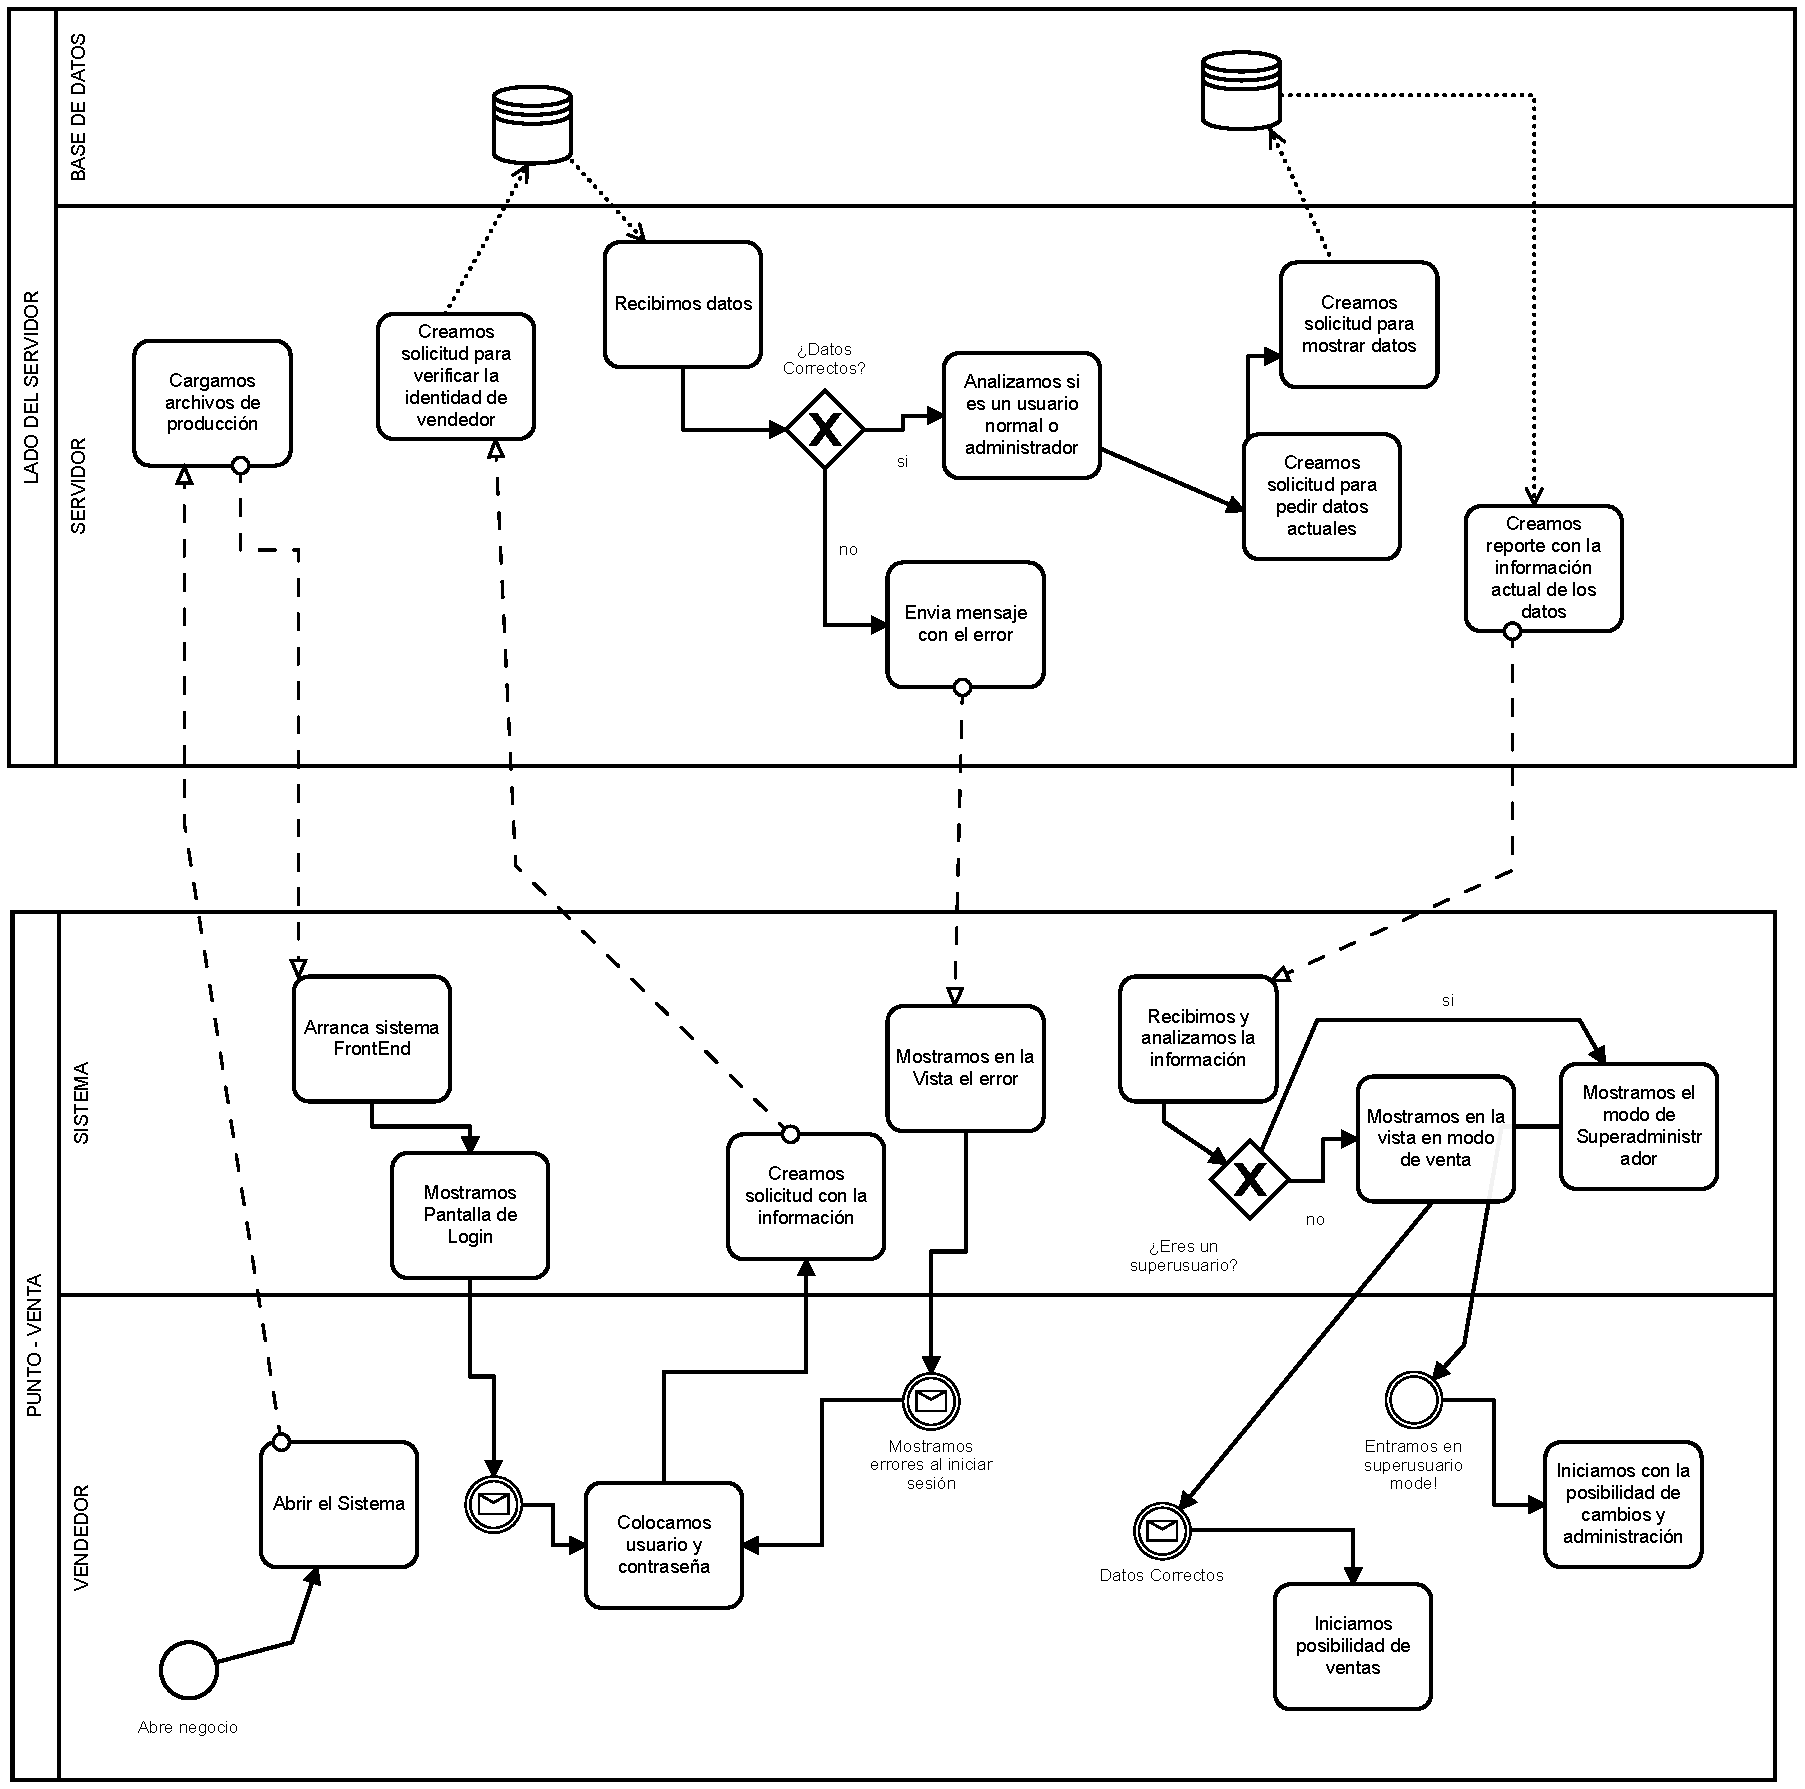
\includepdf[pages=-,pagecommand={},width=\textwidth]{1.pdf}

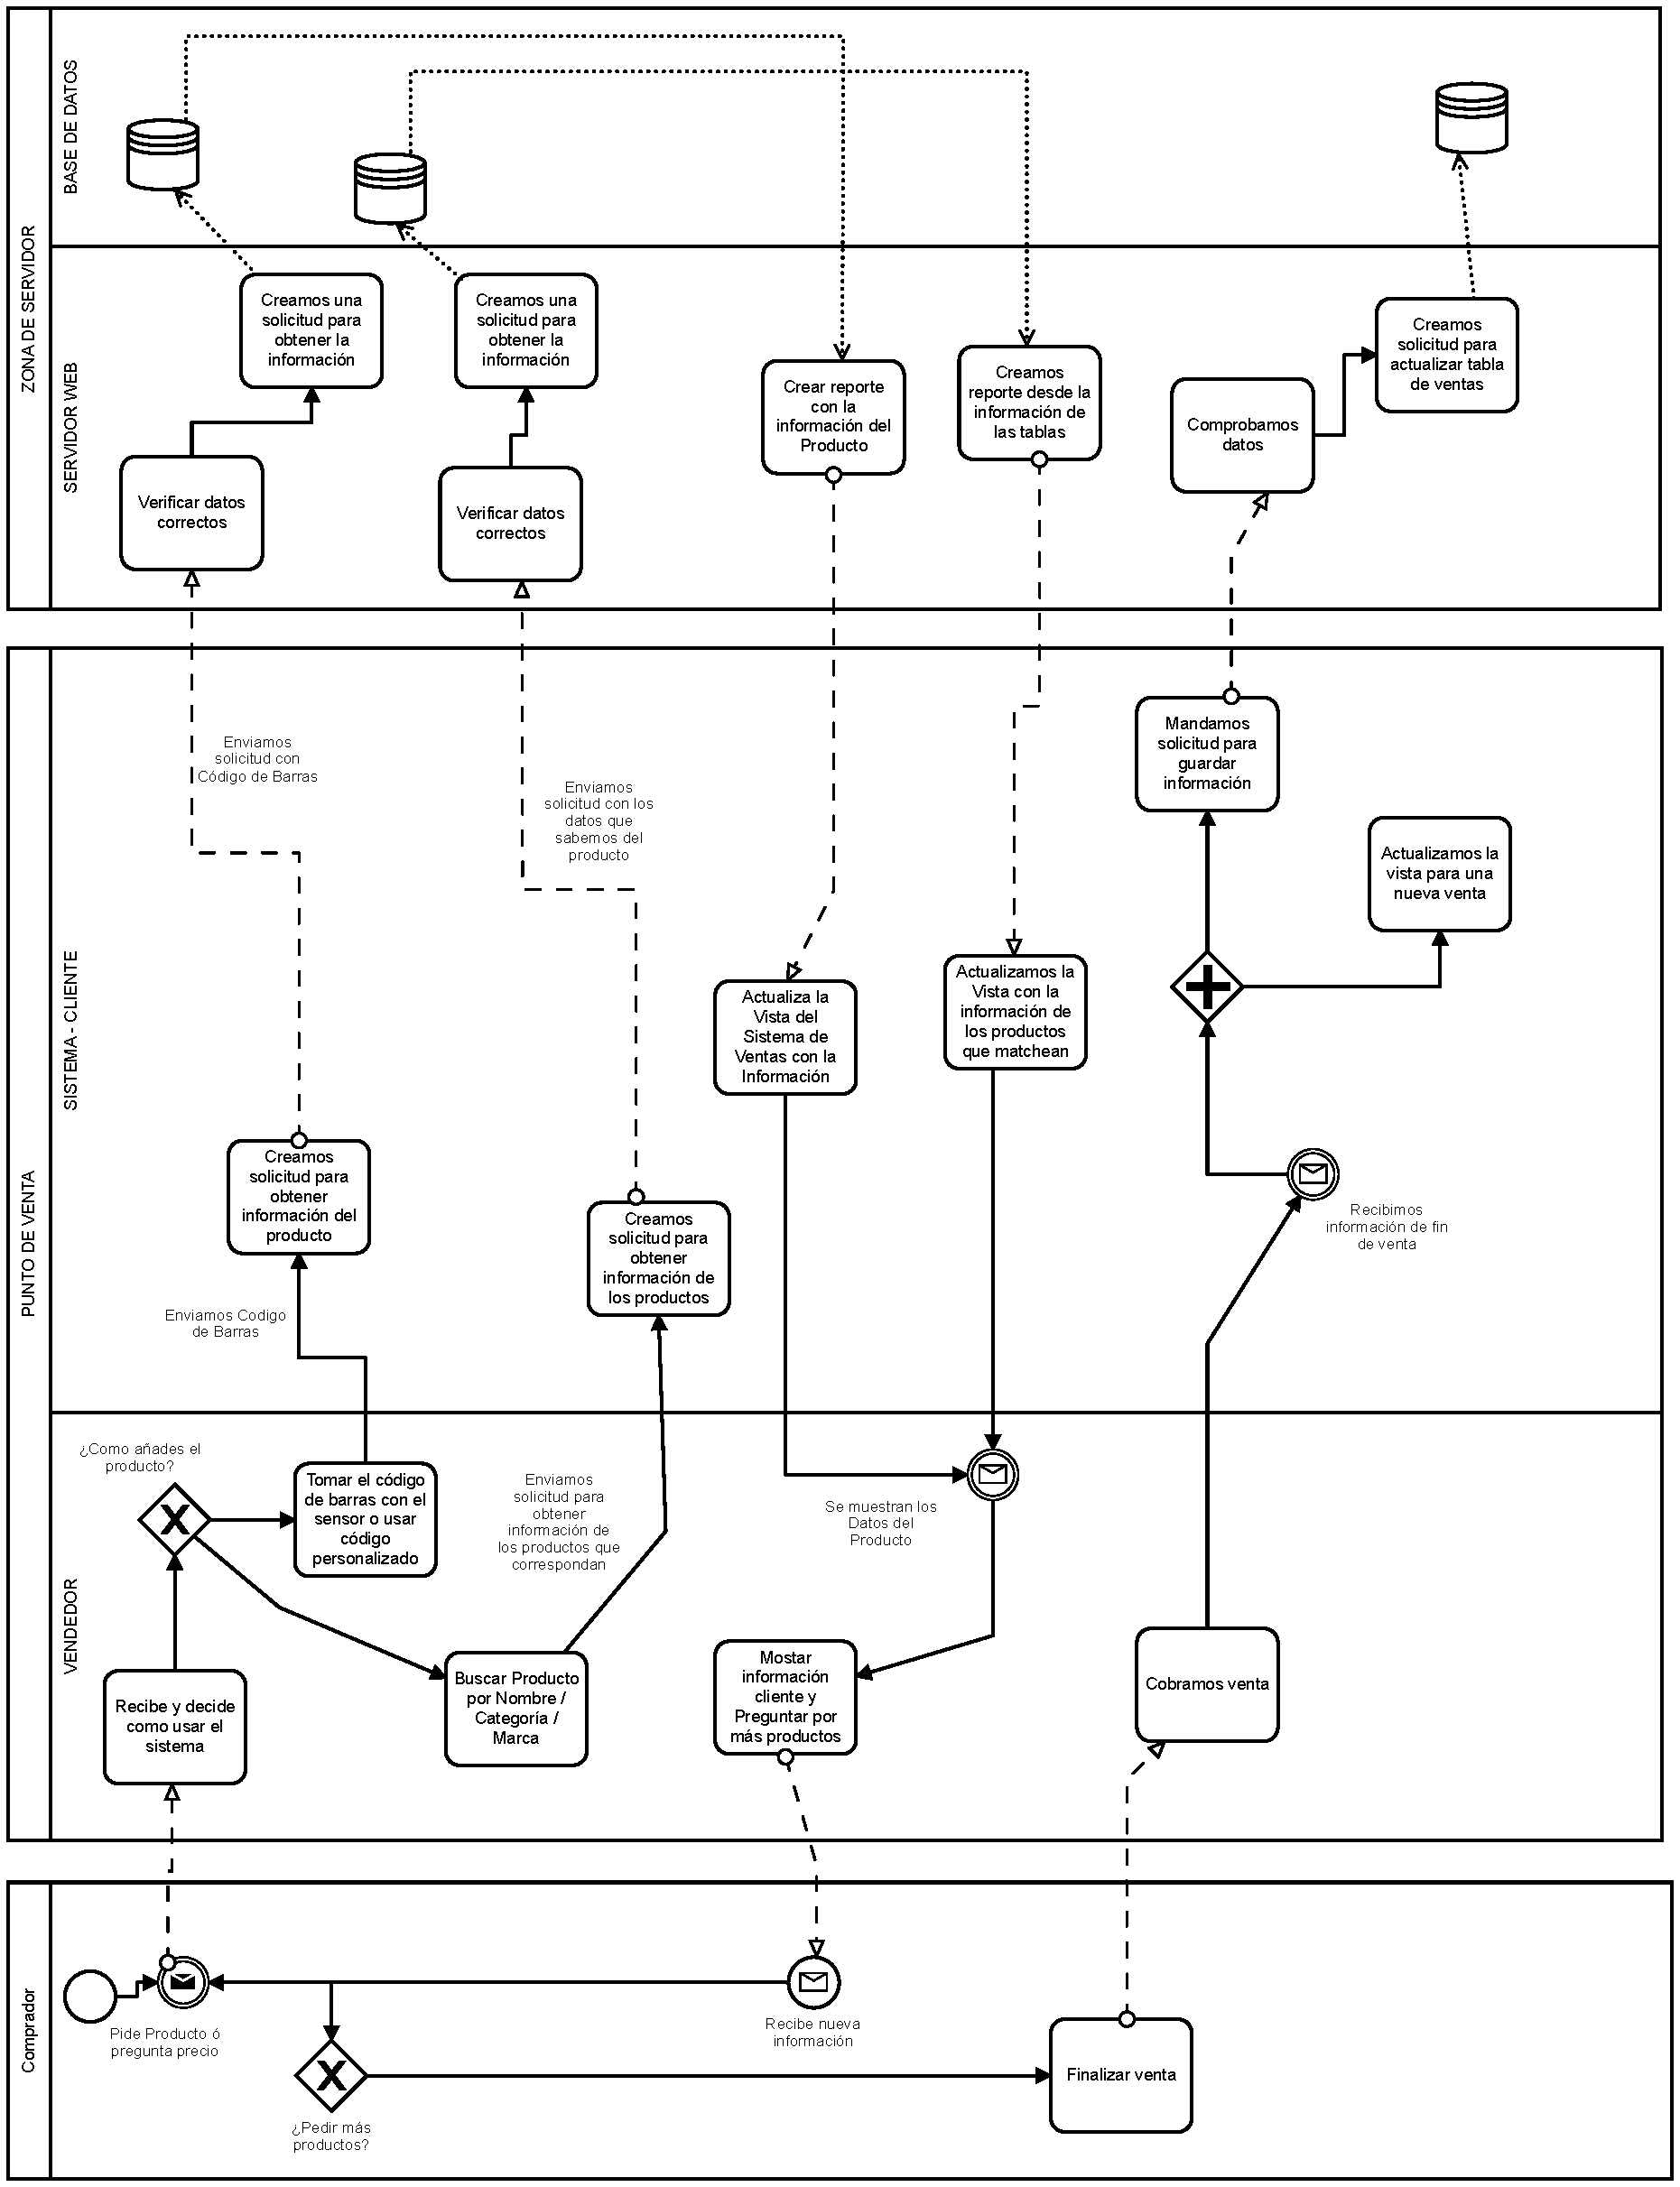
\includepdf[pages=-,pagecommand={},width=\textwidth]{2.pdf}



% ===============================================
% ========        BIBLIO      ===================
% ===============================================
\begin{thebibliography}{10}

    \bibitem{CodeName1} 
        Agile Manifiesto
        \textit{http://agilemanifesto.org/}. 

    \bibitem{CodeName2} 
    	Frank Rosner J, Explain Agile Like I'm a Sports Student 
        \textit{https://dev.to/frosnerd/explain-agile-like-im-a-sports-student-3m8l}. 
        
    \bibitem{CodeName3} 
        Francisco Ruiz, Fac. de Ciencias
        \textit{https://www.ctr.unican.es/asignaturas/is1/is1-t02-trans.pdf}. 

\end{thebibliography}

\end{document}
